% An Overview of Lie Algebra's
% Adapted from Justin Ryan's "Examples of Lie Algebras"
% Chaskin Saroff and Alexander Jansing	
% last changed: 3 May 2015
% feel free to make any improvements/changes you wish

\documentclass[9 pt]{beamer}
\usepackage{etex}
\reserveinserts{32}
% \usepackage{default}
\usepackage{lmodern}
\usepackage{amsmath,amsfonts,epsfig,pgf} % ,graphicx
\usepackage{graphicx}
\usepackage{hyperref}

% choose your theme
 \usetheme{Warsaw} % Warsaw, Copenhagen, Darmstadt, Madrid, Singapore, etc...

% custom SUNY Polytechnic color scheme
\definecolor{polytechnic}{rgb}{0.05,0.1,0.7}
\setbeamercolor*{palette primary}{fg=white, bg=polytechnic}
\setbeamercolor*{palette sidebar primary}{fg=black, bg=polytechnic}
\setbeamercolor{block title}{bg=black,fg=white} % bg=background, fg= foreground
\setbeamercolor{block body}{bg=polytechnic,fg=black} % bg=background, fg= foreground
\setbeamercolor{alerted text}{fg=polytechnic}
\usecolortheme[named={polytechnic}]{structure}
\def\today{\number\day\space\ifcase\month\or
   January\or February\or March\or April\or May\or June\or
   July\or August\or September\or October\or November\or December\fi
   \space\number\year}

% something I found to get alert blocks in the polytechnic color scheme
\newenvironment<>{lakeblock}[1]{%
  \begin{actionenv}#2%
      \def\insertblocktitle{#1}%
      \par%
      \mode<presentation>{%
\setbeamercolor{block title}{fg=white,bg=black}
       \setbeamercolor{block body}{fg=white,bg=polytechnic}
            }%
      \usebeamertemplate{block begin}}
    {\par\usebeamertemplate{block end}\end{actionenv}}

% polytechnic State logo on every page
%\logo{\pgfputat{\pgfxy(-10.5,0.35)}{\pgfbox[center,center]
%{\includegraphics[height=1.35cm]{polytechnic_logo_horiz_grn}}}}

% commutative diagrams with XY-pic
\usepackage[all]{xy}
\SelectTips{cm}{}
% make \mathscr, TeX \cal, and Euler script *all* available
% (notice the new command names to avoid overlap and/or confusion)
\usepackage{mathrsfs}
\let\rscr=\mathscr % use \rscr{} for Ralph Smith fancy script
\let\mathscr=\relax
\let\mcal=\mathcal % use \mcal{} for TeX \cal script
\usepackage{eucal}
\let\escr=\mathcal % use \escr{} for Euler script
\let\mathcal=\relax
% a better "bar" thanks to Donald Arsenau -- see \pbar infra
\usepackage{accents}

% title page information
\title[Paying off your loans effectively]{Paying off your loans effectively}
\author{Alexander Jansing}
\date{\today}

% new math commands
\newcommand{\at}[1]{\emph{\alert{#1}}}
\newcommand{\ad}[1]{\text{ad}_{#1}}
\newcommand{\add}[1]{\ad{#1}^\dagger}
\newcommand{\br}[2]{\left[ #1, #2 \right]}
\newcommand{\bre}{\br{\ }{\,}}
\newcommand{\C}{\mathbb{C}}
\newcommand{\F}{\mathbb{F}}
\newcommand{\h}{\lag{h}}
\newcommand{\inp}[2]{\langle #1, #2 \rangle}
\newcommand{\inpe}{\inp{\ }{\,}}
\newcommand{\lag}[1]{\mfrak{#1}}
\newcommand{\mfrak}[1]{\mathfrak{#1}}
\newcommand{\R}{\mathbb{R}}
\renewcommand{\a}{\alpha}
\newcommand{\surj}{\rightarrow\kern-.82em\rightarrow}
\newcommand{\tQ}{\widetilde{Q}}
\renewcommand{\v}{\lal{v}}
\newcommand{\z}{\lal{z}}
\newcommand{\V}{\mathfrak{g}}
\newcommand{\fg}{\mathfrak{g}}
\newcommand{\fz}{\mathfrak{z}}
\newcommand{\fv}{\mathfrak{v}}
\newcommand{\fh}{\mathfrak{h}}
\newcommand{\QQ}{\mathbb{Q}}
\newcommand{\ZZ}{\mathbb{Z}}
\newcommand{\RR}{\mathbb{R}}
\newcommand{\CC}{\mathbb{C}}
\newcommand{\NN}{\mathbb{N}}
\newcommand{\FF}{\mathbb{F}}
\newcommand{\zvec}{\mathbf{0}}
\newcommand{\lal}[1]{\mathfrak{#1}}
\newcommand{\lan}{\lal{n}}
\newcommand{\lav}{\lal{v}}
\newcommand{\laz}{\lal{z}}
%\renewcommand{\span}[1]{\text{span}\left\{#1\right\}}


% colored text commands
\newcommand{\red}[1]{{\color{red} #1}}
\newcommand{\grn}[1]{{\color{green} #1}}
\newcommand{\blu}[1]{{\color{blue} #1}}
\newcommand{\ylw}[1]{{\color{yellow} #1}}
\newcommand{\mgn}[1]{{\color{magenta} #1}}
\newcommand{\cyn}[1]{{\color{cyan} #1}}

%Stuff from Justin's example
%\renewcommand{\a}{\vect{a}}
%\newcommand{\abs}[1]{\vert #1 \vert}
%\renewcommand{\b}{\vect{b}}
%\newcommand{\bve}{\pbar{\ve}}
%\newcommand{\dps}{\displaystyle}
%\newcommand{\ds}{\oplus}
%\newcommand{\name}{{\bf Name:}\underline{\hspace{3 in}}}
%\newcommand{\nin}{\noindent}
%\newcommand{\norm}[1]{\left\Vert #1 \right\Vert}
%\newcommand{\pg}[1]{\paragraph{#1}}
%\newcommand{\ph}[1]{\phantom{#1}}
%\renewcommand{\span}[1]{\textrm{span}\left\{ #1 \right\}}
\renewcommand{\t}{\texttt{t}}
\newcommand{\T}{\textsc{T}}
\renewcommand{\u}{\vect{u}}
\renewcommand{\v}{\vect{v}}
\newcommand{\ve}{\varepsilon}
\newcommand{\vc}[1]{\left\langle #1 \right\rangle}
\newcommand{\vect}[1]{\mathbf{#1}}

% tiks packages
\usepackage{tikz}
\usetikzlibrary{calc}
\usepackage{tikzscale}
\usepackage{filecontents}
\usepackage{caption}
\usepackage{subcaption}
\captionsetup{compatibility=false}
\usepackage{wrapfig}

\newcommand{\tikzmark}[1]{\tikz[overlay,remember picture] \node (#1) {};}
\newcommand{\DrawBox}[1][]{%
    \tikz[overlay,remember picture]{
    \draw[red,#1]
      ($(left)+(-0.2em,0.9em)$) rectangle
      ($(right)+(0.2em,-0.3em)$);}
}


%%%ENUMERATE OVER SLIDES%%%
\newcounter{sauvegardeenumi}
\newcommand{\asuivre}{\setcounter{sauvegardeenumi}{\theenumi}}
\newcommand{\suite}{\setcounter{enumi}{\thesauvegardeenumi}}
%%%%%%%%%%%%%%%%%%%%%%%%%%%

\NewDocumentCommand{\highlight}{O{blue!40} m m}{%
    \draw[mycolor=#1] (#2.north west)rectangle (#3.south east);
}

\NewDocumentCommand{\fhighlight}{O{blue!40} m m}{%
    \draw[myfillcolor=#1] (#2.north west)rectangle (#3.south east);
}

\begin{document}

\section{Introduction}


\begin{frame}{}
\vspace{.8 cm}

\titlepage
\begin{center}

\includegraphics[height=2cm]{suny_poly}
\end{center}

\end{frame}

\begin{frame}
Most people have a variety of debts and they can't just pay them off by the end of each month. This lends to the question, "What is the most efficient way to pay off one's debts?"\pause
\begin{enumerate}
\item[] Minimum payments? \pause
\item[]	Max interest first? \pause
\item[] Proportion based on interest rate? \pause
\item[] Proportion based on interest rate and the amount you owe on each debt?
\end{enumerate}
\end{frame}


\section{Methods}
\subsection{Minimum Payments Only}
\begin{frame}
Paying off the minimums every month is obviously the worst method possible, because minimum payments are calculated based your monthly interest plus one to three percent of your principal;
$$minimum = (P*R)*(P*.03)$$
\begin{center}
\href{http://www.creditcards.com/calculators/minimum-payment.php
}{(\blu{source: creditcards.com})}
\end{center}
\end{frame}

\subsection{Paying off Max interest only}
\begin{frame}
The general rule of thumb people usually follow is because of its simplicity; paying off loans with the highest interest rates first. because of my experiences with optimization methods in linear programming, I claim that this method is not the most efficient.
\end{frame}

\subsection{Proportion based solely on interest rates}
\begin{frame}
This method gets closer to what I'm looking for. \pause \\
Given $n$ debts, each debt has a rate $r$. The rates are proportioned as $p_{r_i} = \frac{r_i}{\sum_{j=0}^{n-1}r_j}$. And from here your additional payment will be proportioned out based on what percent that interest rate consisted of in all of your debts.\pause
\begin{center}
\emph{i.e.} If $r_0 = .05$ and $r_1 = .10$, the proportions would be $\frac{1}{3}$ to the first debt and $\frac{2}{3}$ to the second debt and you'd end up paying 33 cents out of every dollar to the first and 67 cents to the second.
\end{center}
\pause
But this seems too simplistic to me, perhaps if we try to distribute the pay some other way?
\end{frame}


\subsection{Proportion based on interest rates and size of debt}
\begin{frame}
This method is as far as I went into searching for how to pay off your loans in an effective way. \pause \\
Given $n$ debts, each debt has a balance $b$ and rate $r$. The rates are proportioned as $p_{r_i} = \frac{r_i}{\sum_{j=0}^{n-1}r_j}$ and similarly the balances are proportioned as $p_{b_i} = \frac{b_i}{\sum_{j=0}^{n-1}b_j}$. And from here your additional payment will be proportioned out based on the individual interest rate percentage multiplied by the percent of the total a certain debt made up.\pause
$$p_{r_i}*b_{b_i}*(extraAmountPayoff)$$
\pause
\end{frame}

\section{Analysis}
\subsection{Running Time}
\begin{frame}
I created a shell script that ran the program against various \emph{extraAmountPayoff} amounts; \textsc{pay.sh}.
In the latest iteration of the program, the following times were recorded for running times:\\
$
\begin{array}{c|c|c}
extraAmountPayoff&Serial (seconds) &Parallel (seconds)\\
10&0.0123219490051&0.00575304031372\\
100&0.00804305076599&0.00271987915039\\
1000&0.0045371055603&0.00170397758484\\
10000&0.00340819358826&0.00142216682434\\
\end{array}
$
\end{frame}

\subsection{Amounts paid}
\begin{frame}
\begin{center}
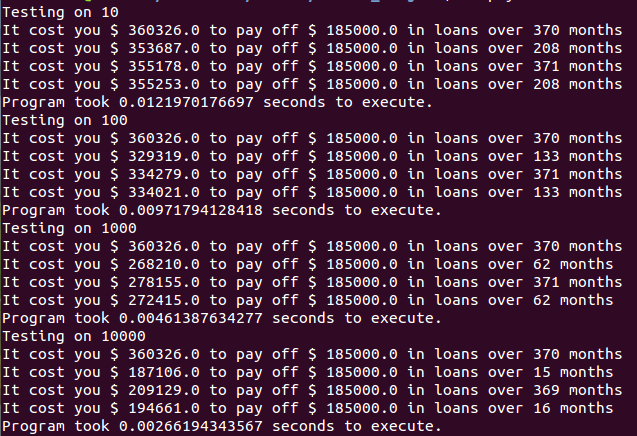
\includegraphics[height = 4.5cm]{payOffs}
\end{center}
\end{frame}

\end{document}
















